\documentclass[11pt]{beamer}

% use utf8 instead of latin1 when using LaTeX in windows
\usepackage[utf8]{inputenc}

%ds custom packages
%\usepackage{cleveref}
\usepackage{empheq}
\usepackage{graphicx}
\usepackage[font={small}]{caption}
\usepackage{subcaption}
\usepackage{framed}
\usepackage{listings}
\usepackage{wrapfig}
\usepackage{sidecap}
\usepackage{xcolor}
\usepackage{lineno}
\usepackage{marvosym}
\usepackage{xstring}
\usepackage{mfirstuc}
\usepackage{hyperref}

\lstset { %
    language=C++,
    backgroundcolor=\color{black!5}, % set backgroundcolor
    basicstyle=\footnotesize,% basic font setting
}

%ds colors
\definecolor{orange}{rgb}{1,0.4,0}
\definecolor{green}{rgb}{0,0.5,0}

%ds referencing
\newcommand{\myref}[3]{\hyperref[#1]{#2} (\capitalisewords{#3} \ref{#1})}

%ds blue box
\definecolor{myblue}{rgb}{.9, .9, 1}

\newlength\mytemplen
\newsavebox\mytempbox
\newcommand*\widefbox[1]{\fbox{\hspace{2em}#1\hspace{2em}}}

\makeatletter
\newcommand\mybluebox{%
    \@ifnextchar[%]
       {\@mybluebox}%
       {\@mybluebox[0pt]}}

\def\@mybluebox[#1]{%
    \@ifnextchar[%]
       {\@@mybluebox[#1]}%
       {\@@mybluebox[#1][0pt]}}

\def\@@mybluebox[#1][#2]#3{
    \sbox\mytempbox{#3}%
    \mytemplen\ht\mytempbox
    \advance\mytemplen #1\relax
    \ht\mytempbox\mytemplen
    \mytemplen\dp\mytempbox
    \advance\mytemplen #2\relax
    \dp\mytempbox\mytemplen
    \colorbox{myblue}{\hspace{1em}\usebox{\mytempbox}\hspace{1em}}}

%ds global definitions
\def\P{\mathcal P}
\def\tab{\phantom{tab}}
\def\homx{\mathbf{\tilde{x}}}
\def\trans{\mathbf{t}}
\def\quat{\mathbf{q}}
\renewcommand{\thesubfigure}{\arabic{subfigure}}

%ds set background template
\usebackgroundtemplate
{
    
\includegraphics[width=\paperwidth]{figures/slides.pdf}%
}

%ds disable controls on slides
\setbeamertemplate{navigation symbols}{}

%ds info
\title{Online large-scale SLAM with stereo visual-inertial sensors}
\author{Dominik Schlegel}
\date{\today}

%ds redefine footline
\makeatother
\setbeamertemplate{footline}
{
  \leavevmode%
  \hbox{%
  \hspace{10pt}
  \begin{beamercolorbox}[wd=.6\paperwidth,ht=2.25ex,dp=1ex,center]{author in head/foot}%
    \textcolor{white}{\hspace{60pt}\inserttitle}
  \end{beamercolorbox}%
  \begin{beamercolorbox}[wd=.4\paperwidth,ht=2.25ex,dp=1ex,center]{title in head/foot}%
    \textcolor{white}{\insertdate}\hspace*{3em}
    \textcolor{white}{\insertframenumber{}}\hspace*{1ex}
  \end{beamercolorbox}}%
  \vspace{10pt}%
}
\makeatletter

\begin{document}

%ds titlepage
{
\setbeamertemplate{footline}{} 
\usebackgroundtemplate{
\includegraphics[width=\paperwidth]{figures/titlepage.pdf}}
\begin{frame}
\vspace{-70pt}
\center{\Huge{\textcolor{white}{\inserttitle}}}\\
\vspace{20pt}
\begin{minipage}{1.07\textwidth}
\textcolor{white}{\hfill\small{\insertauthor}}\\
\textcolor{white}{\hfill\small{Supervisor: Prof. Dr. Giorgio Grisetti}}
\end{minipage}
\vspace{10pt}\\
\hspace{-25pt}\textcolor{white}{\small{\insertdate}}
\end{frame}
}

\setcounter{framenumber}{0}

\begin{frame}{Our mission}
\begin{figure}[!htb]
\centering
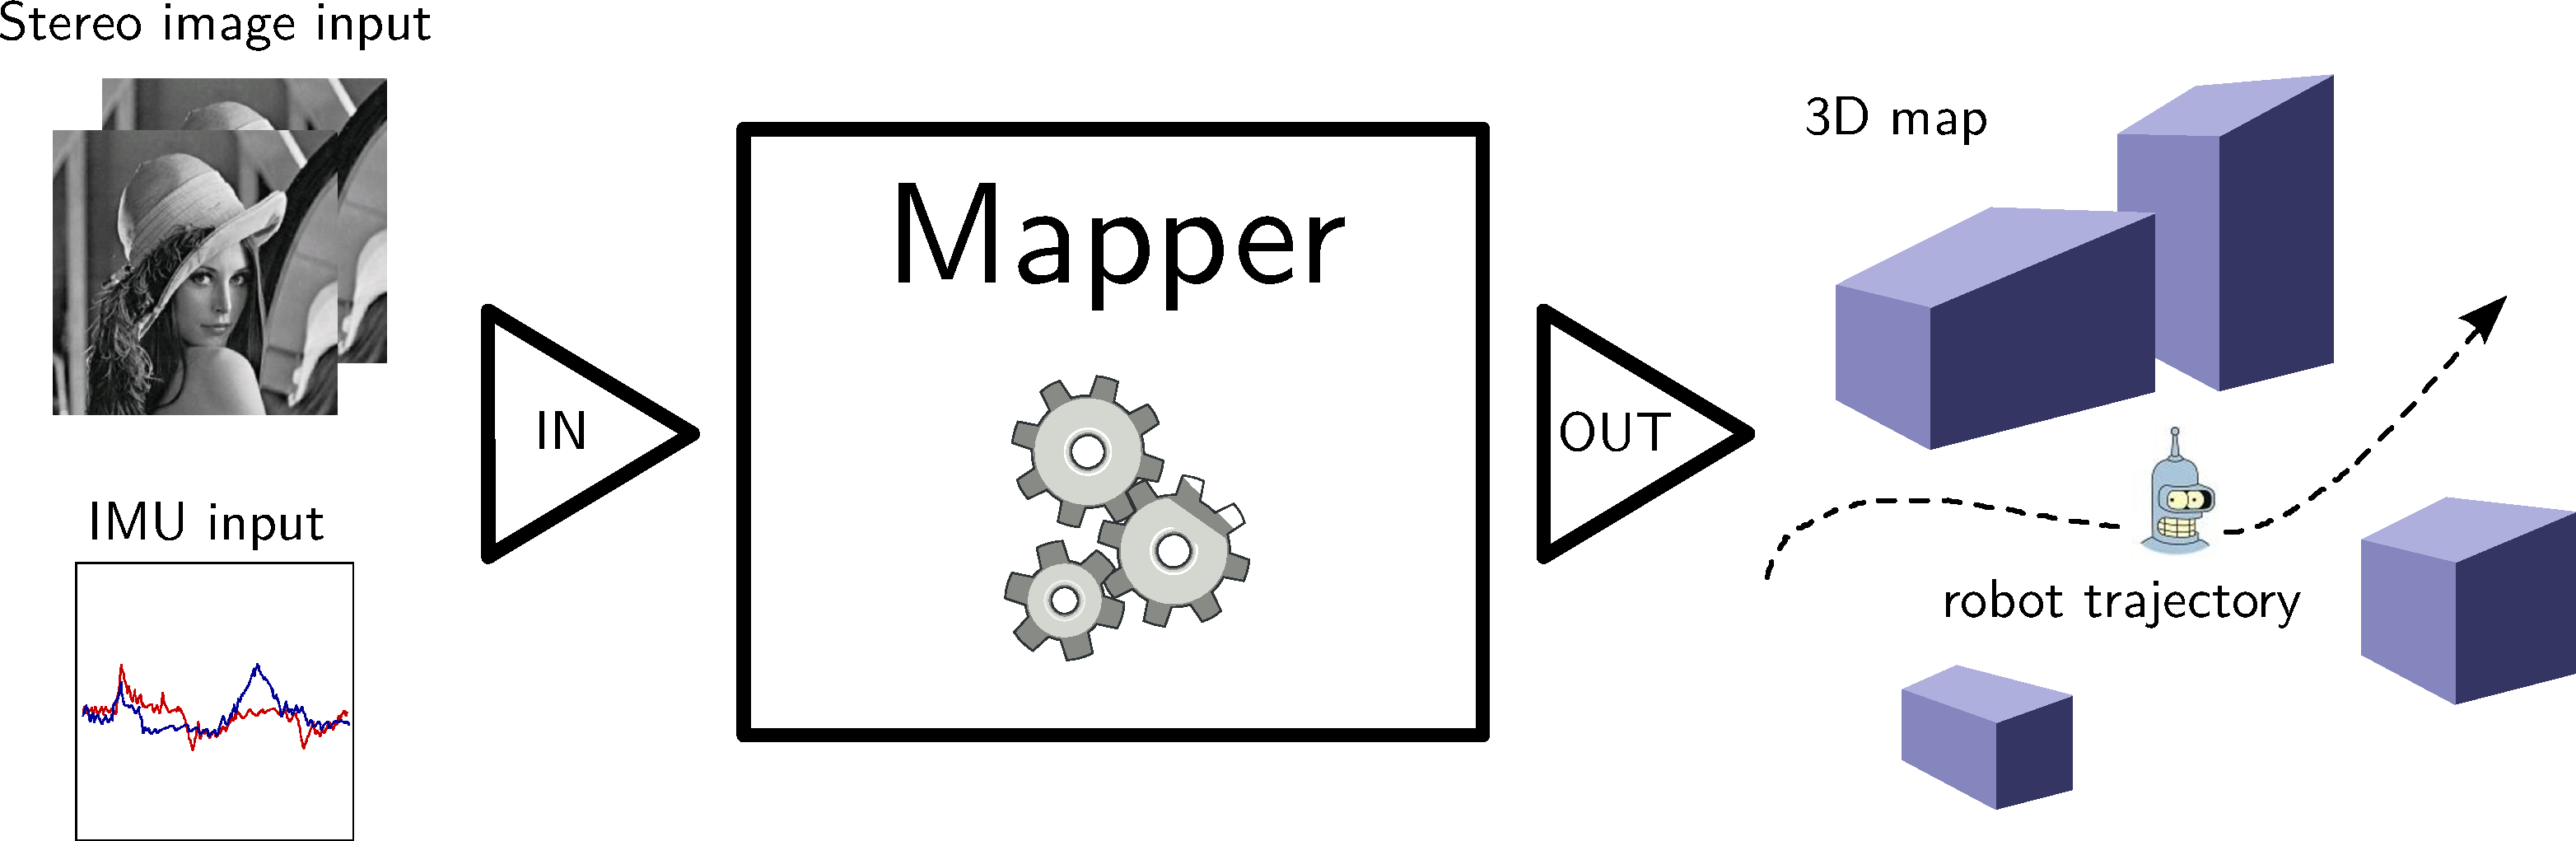
\includegraphics[width=\textwidth]{figures/introduction/basic_concept.pdf}
\end{figure}
Required capabilities:
\begin{itemize}
\item Tracking (Landmark generation, Odometry)
\item Local mapping (Key frame generation, Loop closing)
\item Global mapping (Solving SLAM problem)
\end{itemize}
\end{frame}
\begin{frame}{Related work and state of the art}
Google (street) mapping
\begin{figure}[!htb]
\centering
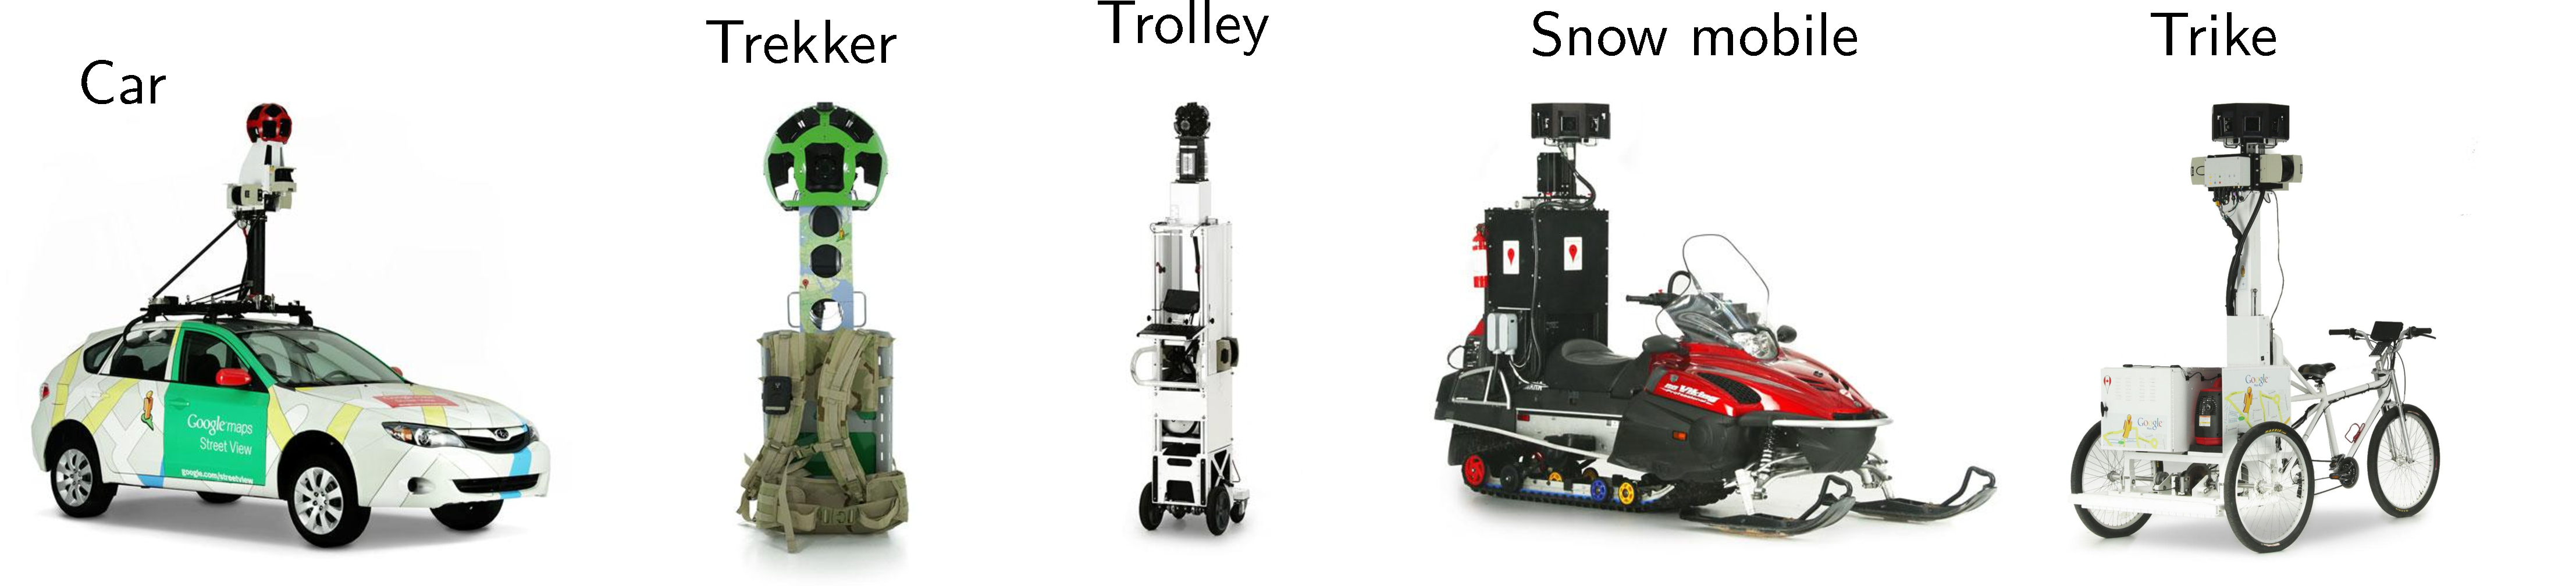
\includegraphics[width=\textwidth]{figures/introduction/google_fleet.pdf}
\vspace{10pt}
\begin{subfigure}[b]{0.45\textwidth}
ORB-SLAM (Mur-Artal et al)
 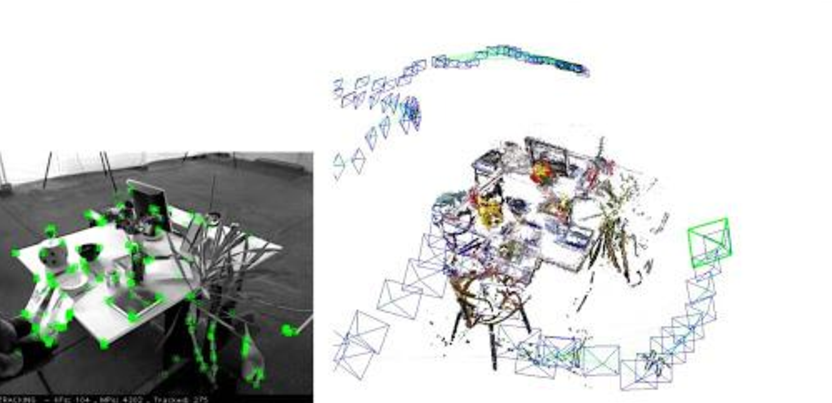
\includegraphics[width=\textwidth]{figures/introduction/ORB_SLAM.pdf}
\end{subfigure}
\hfill
\begin{subfigure}[b]{0.4\textwidth}
ROVINA (Grisetti et al)
 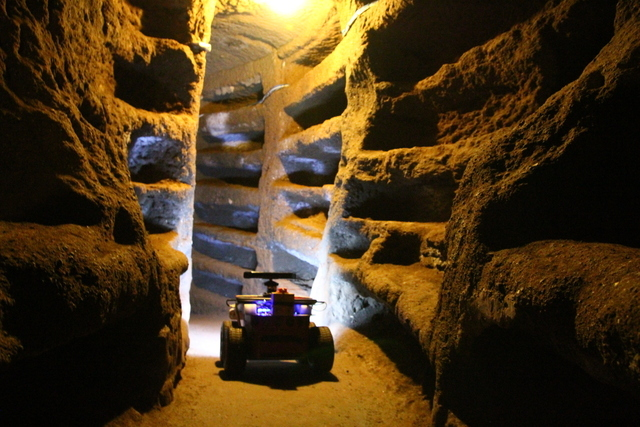
\includegraphics[width=\textwidth]{figures/introduction/ROVINA.jpg}
\end{subfigure}
\end{figure}
\end{frame}
\begin{frame}
\frametitle{Graph-based SLAM}
\begin{figure}[!htb]
\centering
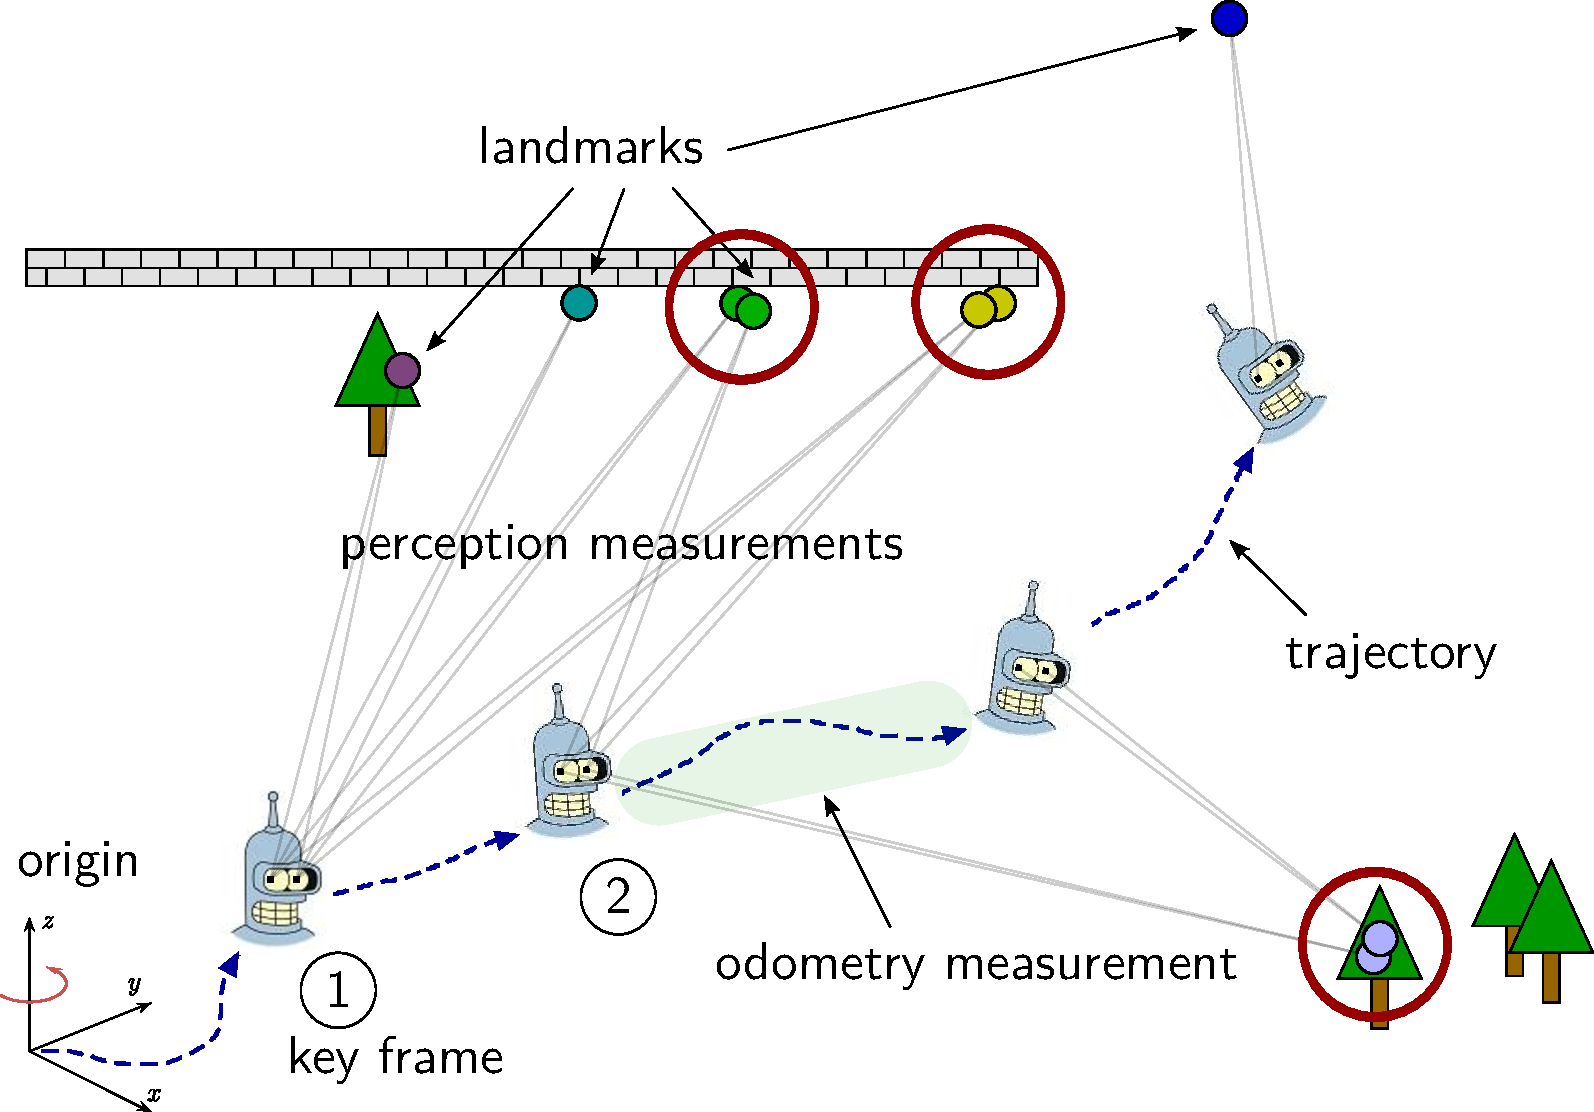
\includegraphics[height=0.925\textheight]{figures/approach_fundamentals/overview_graphslam_simplified.pdf}
\end{figure}
\end{frame}

\begin{frame}{Sensor setup: the VI-Sensor}
\begin{figure}[!htb]
\centering
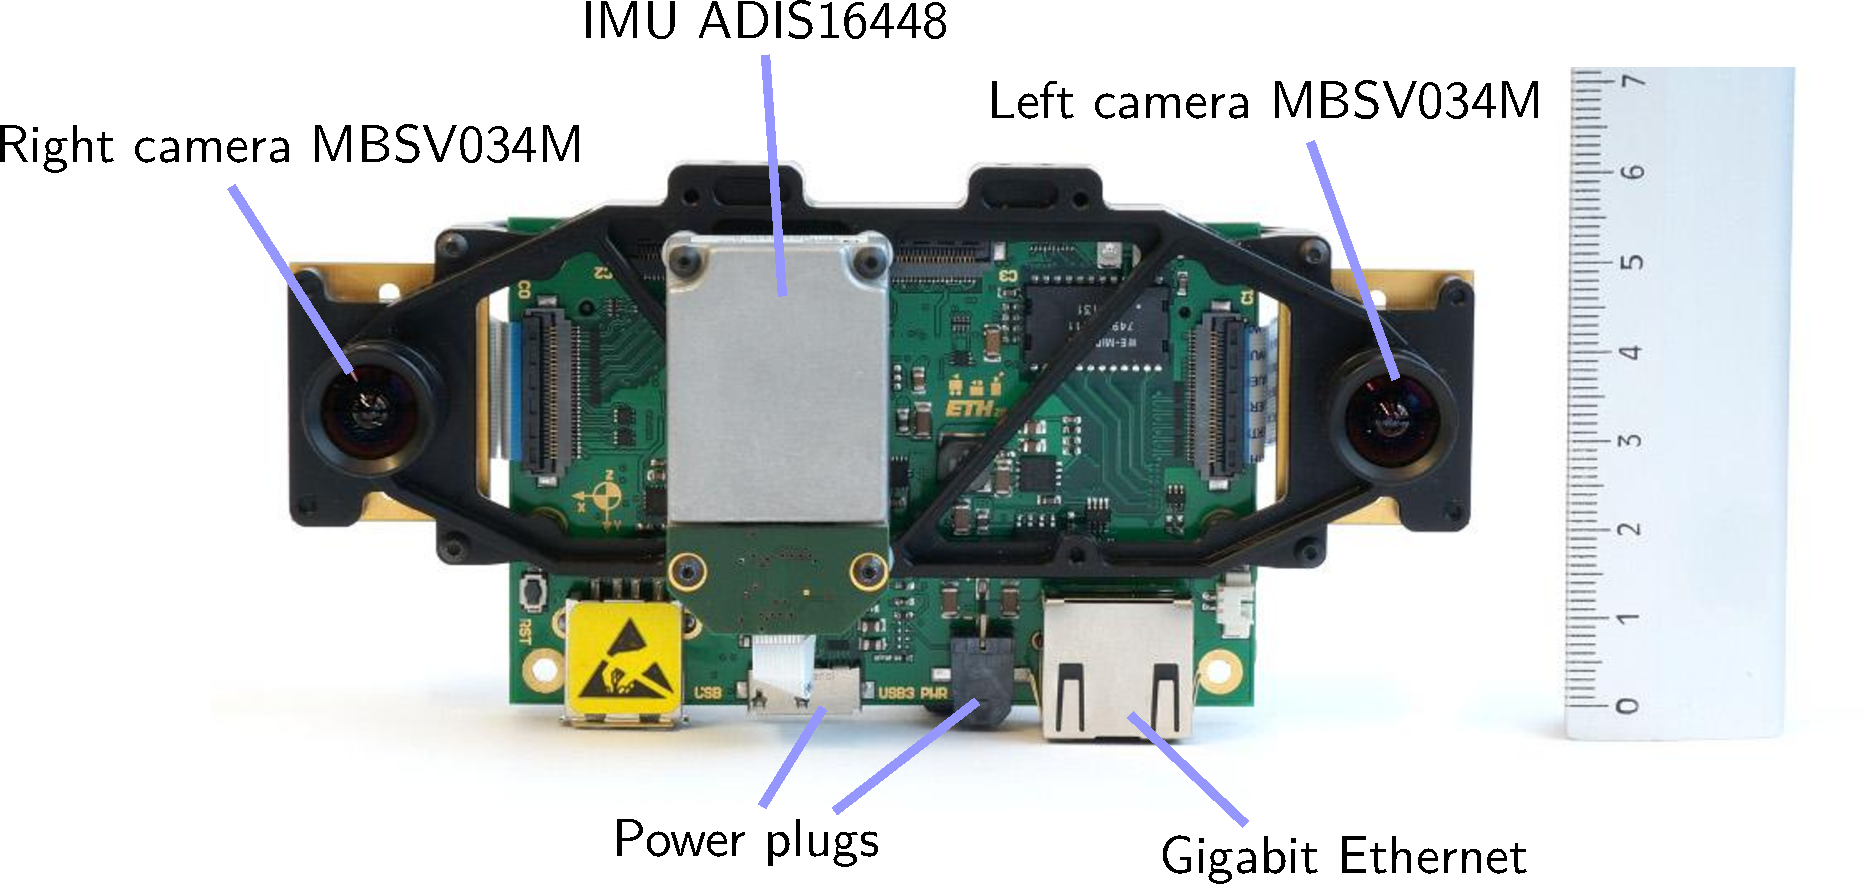
\includegraphics[width=\textwidth]{figures/introduction/vi_sensor_details.pdf}
\end{figure}
\end{frame}

\begin{frame}{First steps}
\begin{figure}[!htb]
\centering
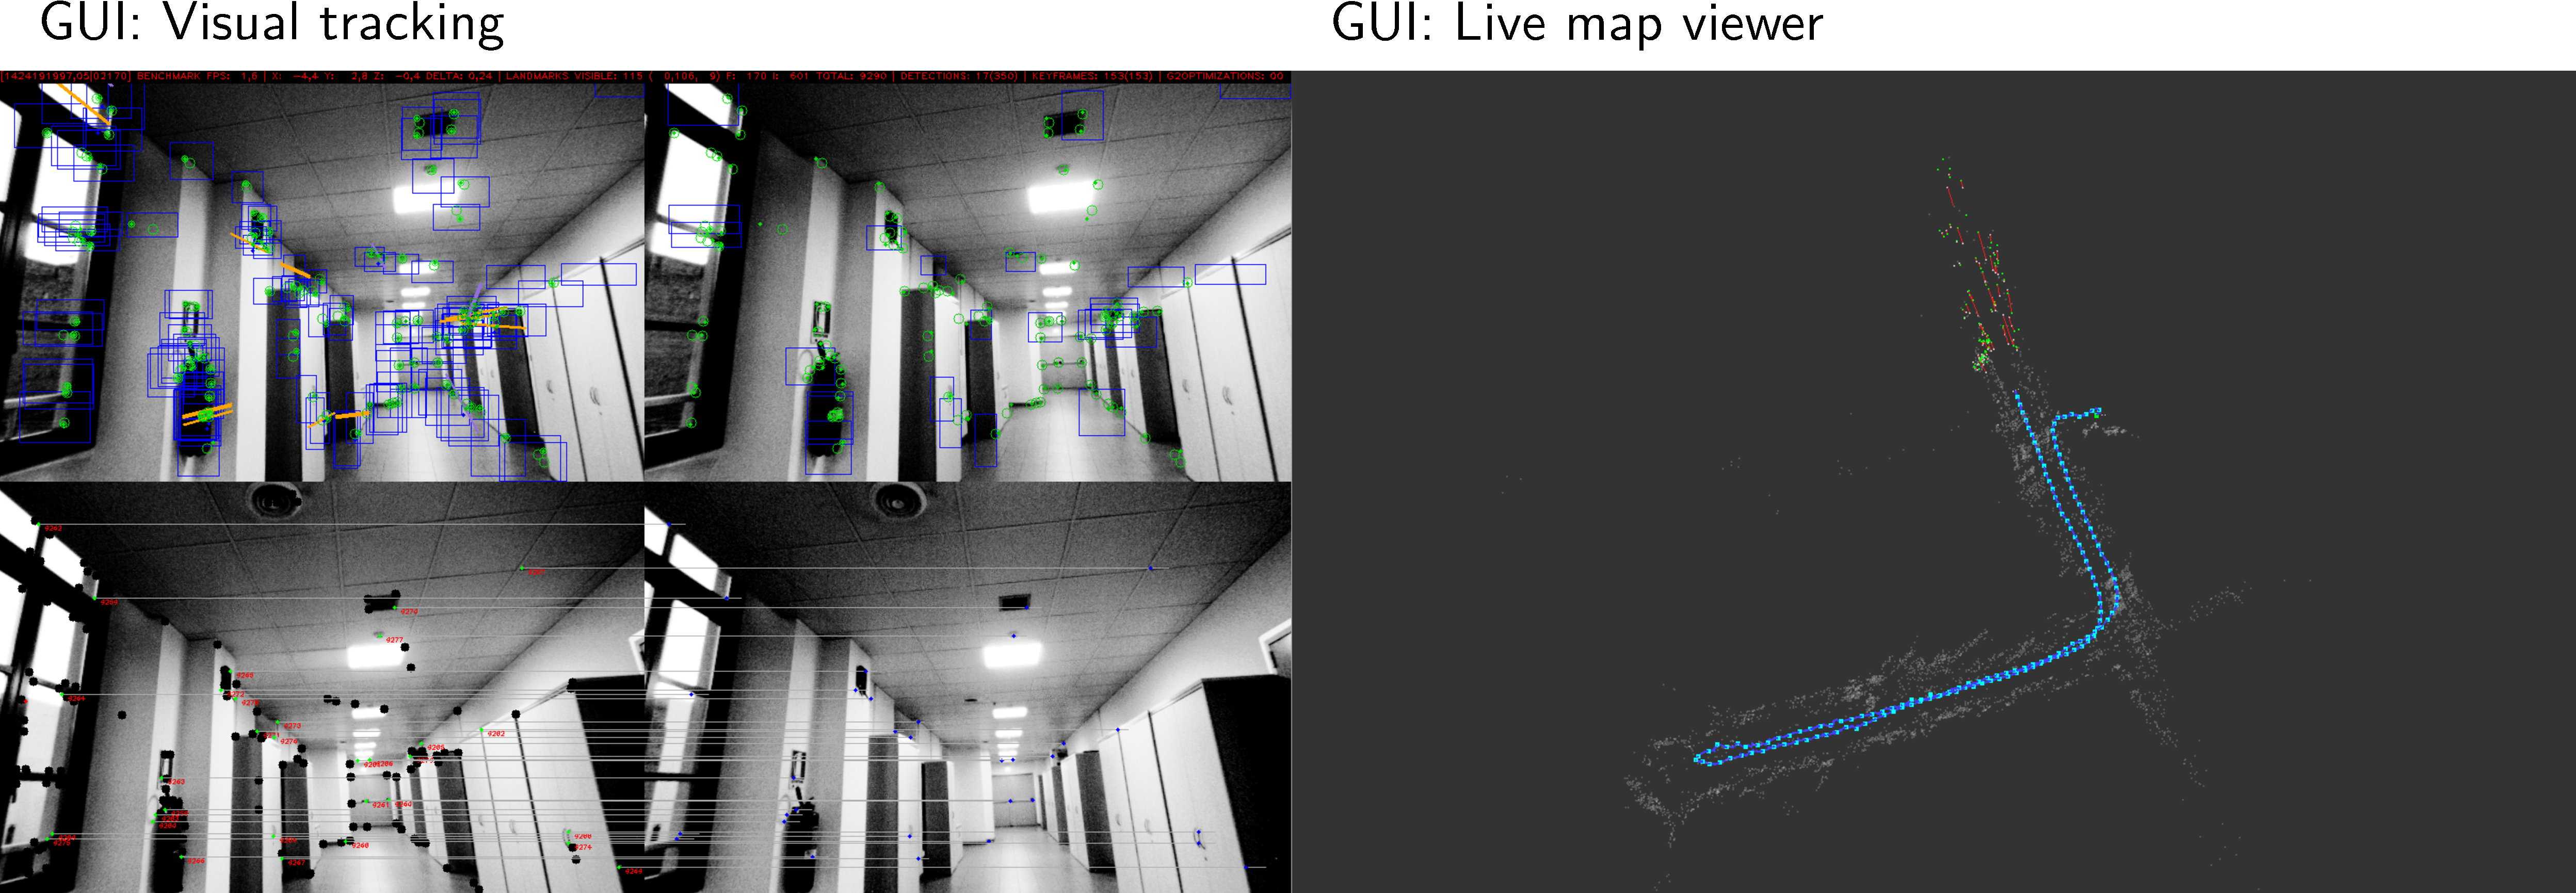
\includegraphics[width=\textwidth]{figures/introduction/first_steps.pdf}
\end{figure}
Many simplifications:
\begin{itemize}
\item Indoor datasets with slow steady movement
\item Odometry by Alberto\texttrademark
\item Minimal range and disturbance
\end{itemize}
\end{frame}

\begin{frame}{Least squares state optimization}
\begin{itemize}
\item StereoUV $\to$ Landmark position\\\vspace{5pt}
\hspace{10pt}State: Positions $\mathbf{x}(x,y,z)$\\
\hspace{10pt}Measurements: Projections $p_L,p_R$\\
\vspace{10pt}
\item StereoPosit $\to$ Odometry\\\vspace{5pt}
\hspace{10pt}State: Transformation $T_{21}(R,\mathbf{t})$\\
\hspace{10pt}Measurements: Positions $\mathbf{x}$, projections $p_L,p_R$\\
\vspace{10pt}
\item ICP (Besl et al) $\to$ Loop closures\\\vspace{5pt}
\hspace{10pt}State: Transformation $T_{BA}$\\
\hspace{10pt}Measurements: Positions $\mathbf{x}_A,\mathbf{x}_B$\\
\vspace{10pt}
\end{itemize}
\end{frame}

\begin{frame}{g2o: graph-based SLAM optimization (Kümmerle et al)}
\begin{figure}[!htb]
\centering
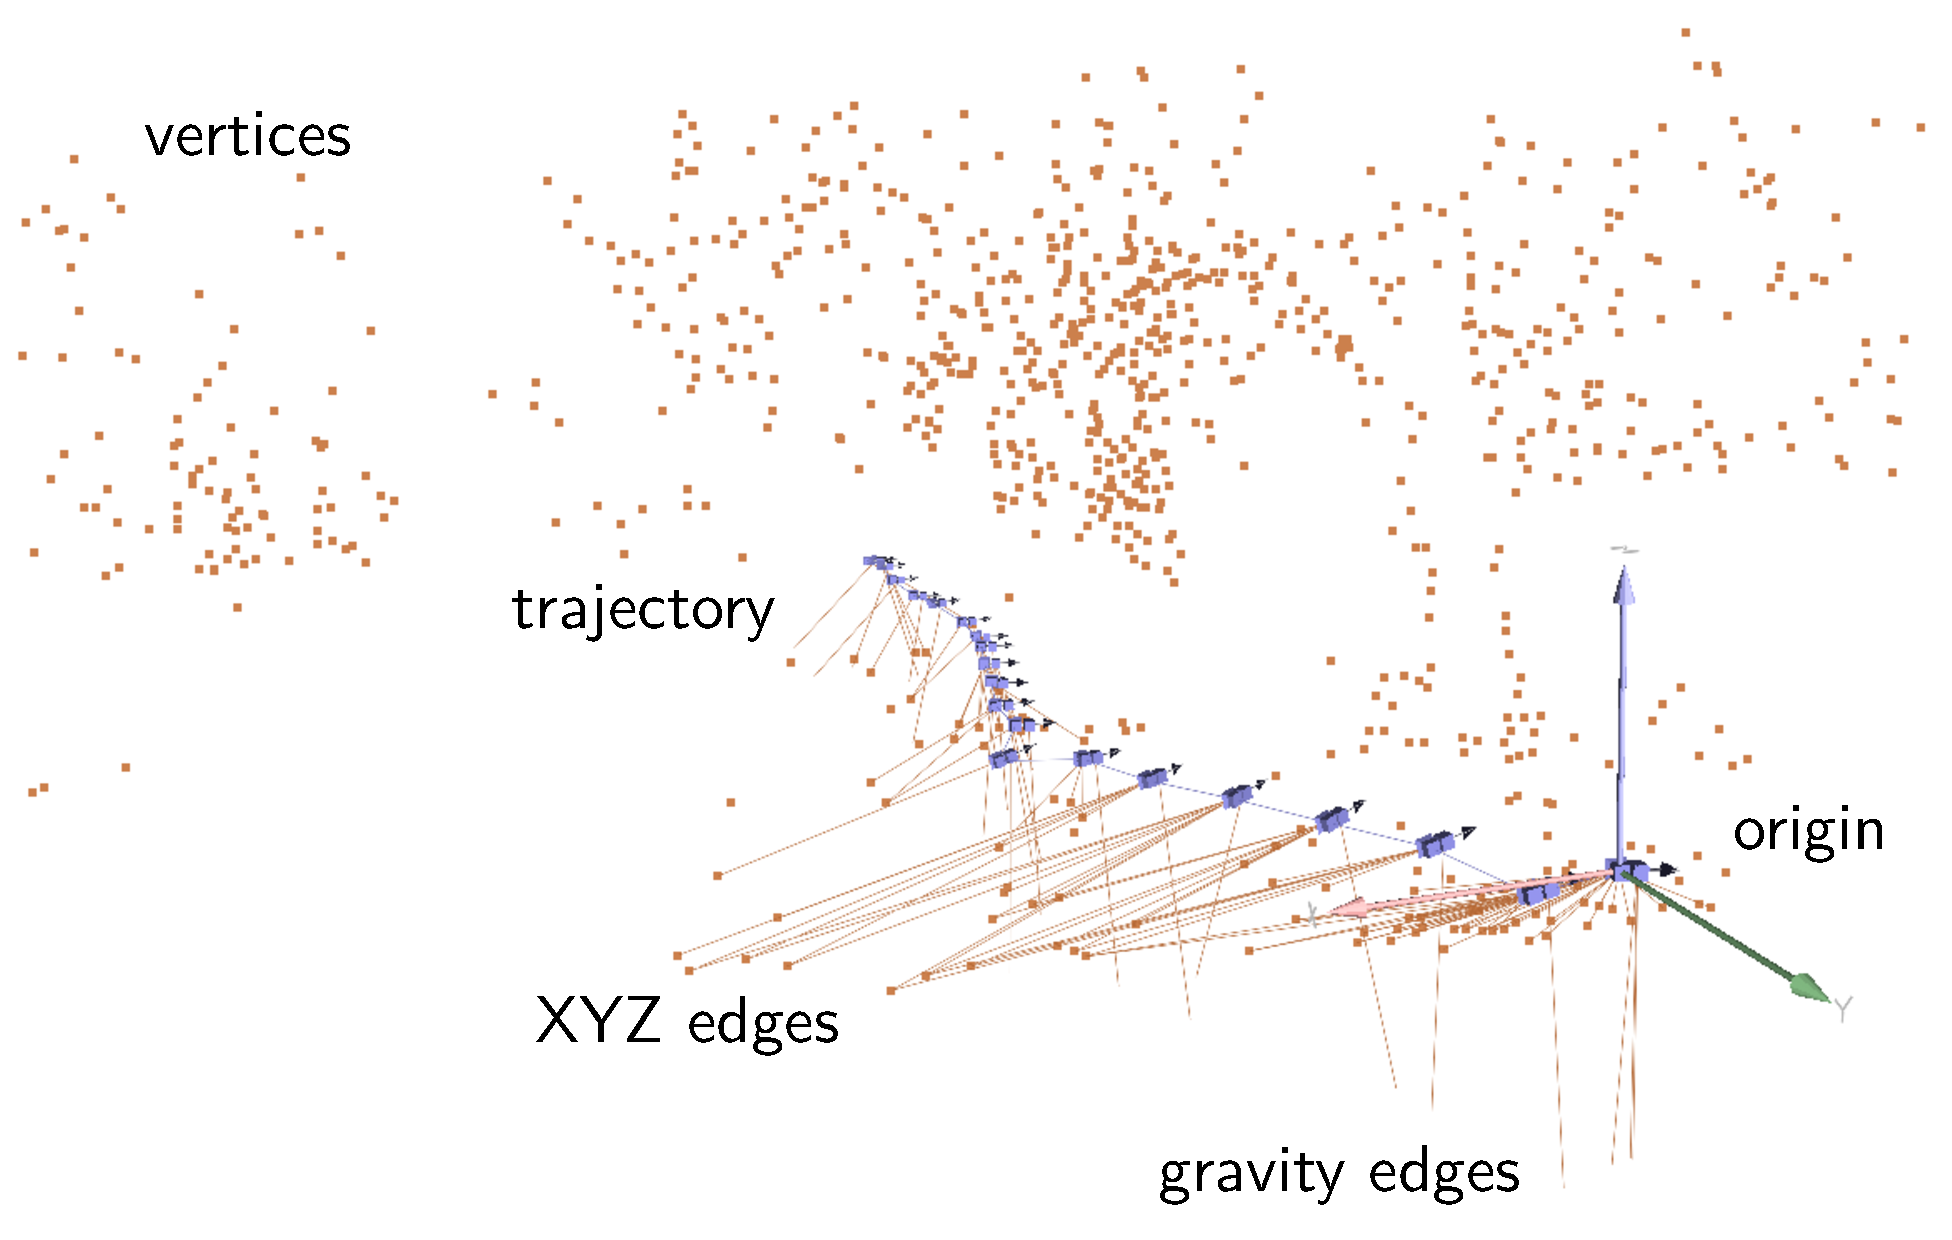
\includegraphics[width=0.95\textwidth]{figures/introduction/g2o_viewer.pdf}
\end{figure}
\end{frame}

\begin{frame}
\frametitle{System in action}
Hand-held dataset: \href{run:/home/n551jw/Documents/presentation_ma/aula_magna.ogv}{Aula Magna}
\begin{figure}[!htb]
\centering
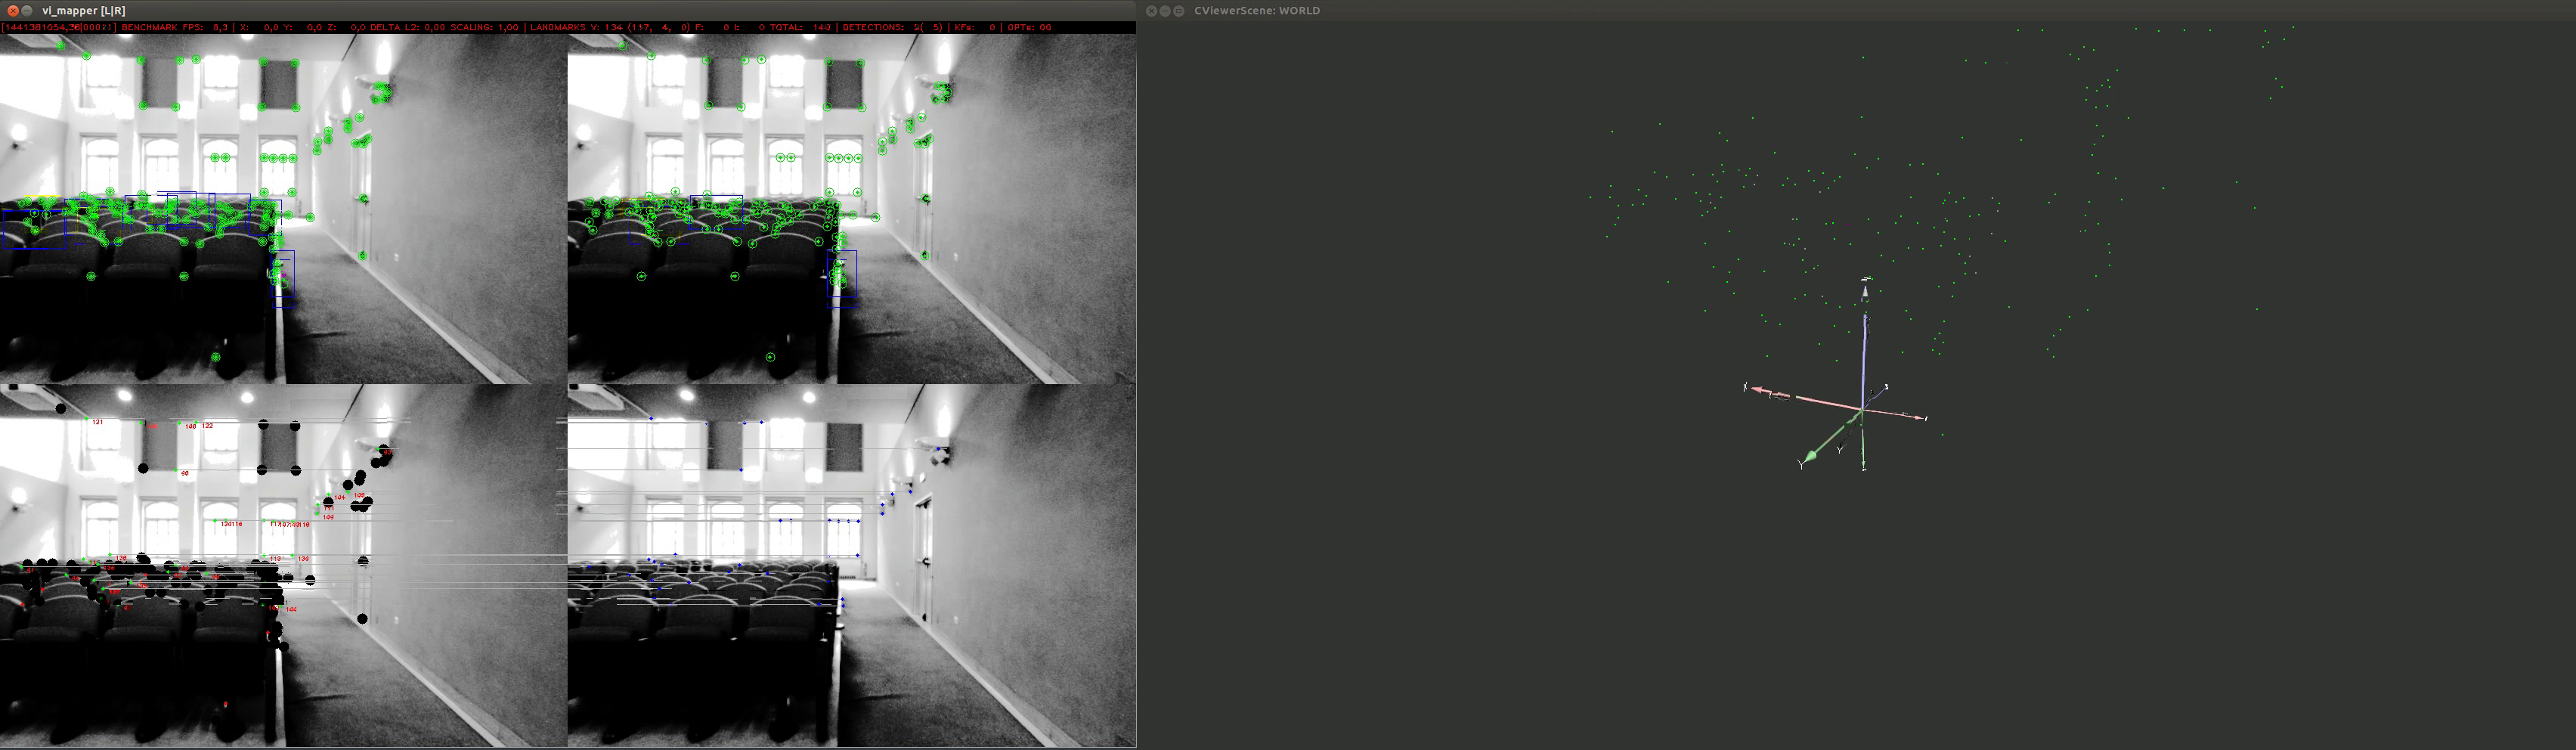
\includegraphics[width=0.87\textwidth]{figures/movie_aula_magna.png}
\end{figure}
Bike mounted dataset: Streets in San Lorenzo
\begin{figure}[!htb]
\centering
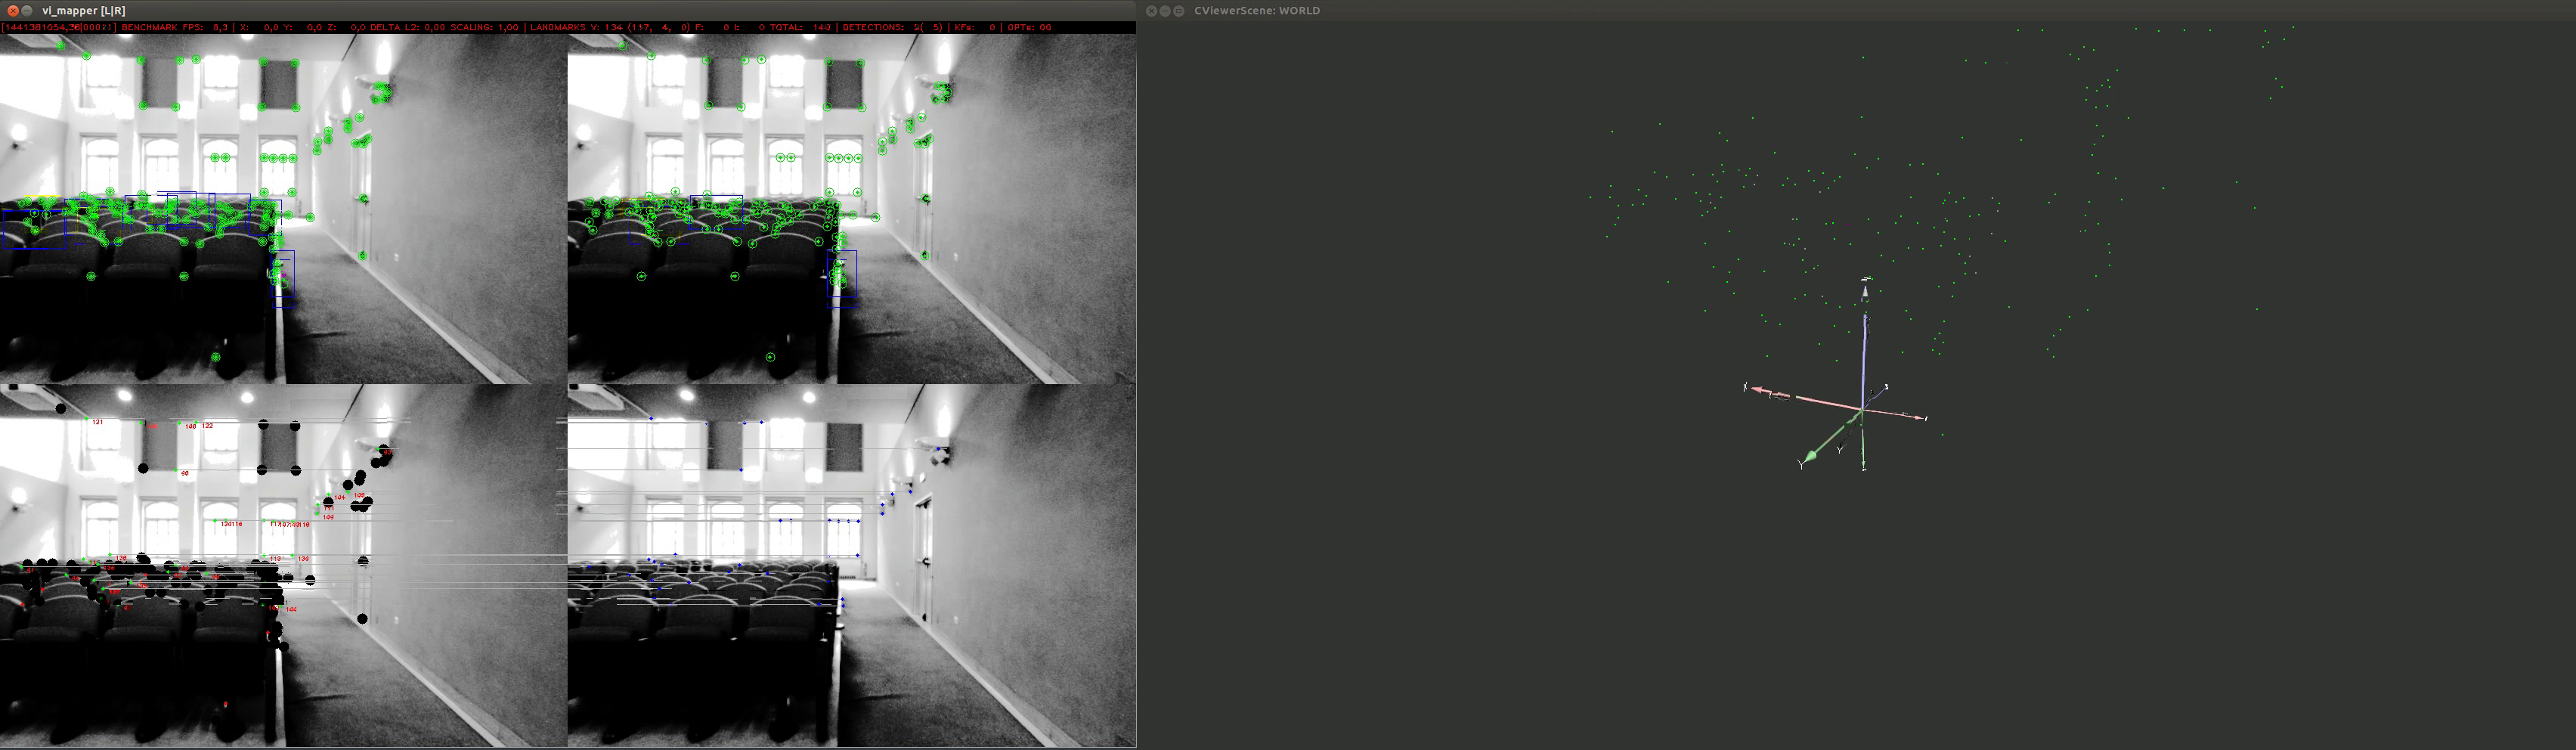
\includegraphics[width=0.87\textwidth]{figures/movie_aula_magna.png}
\end{figure}
\end{frame}

\begin{frame}
\frametitle{Results: hand-held}
\begin{figure}[!htb]
\centering
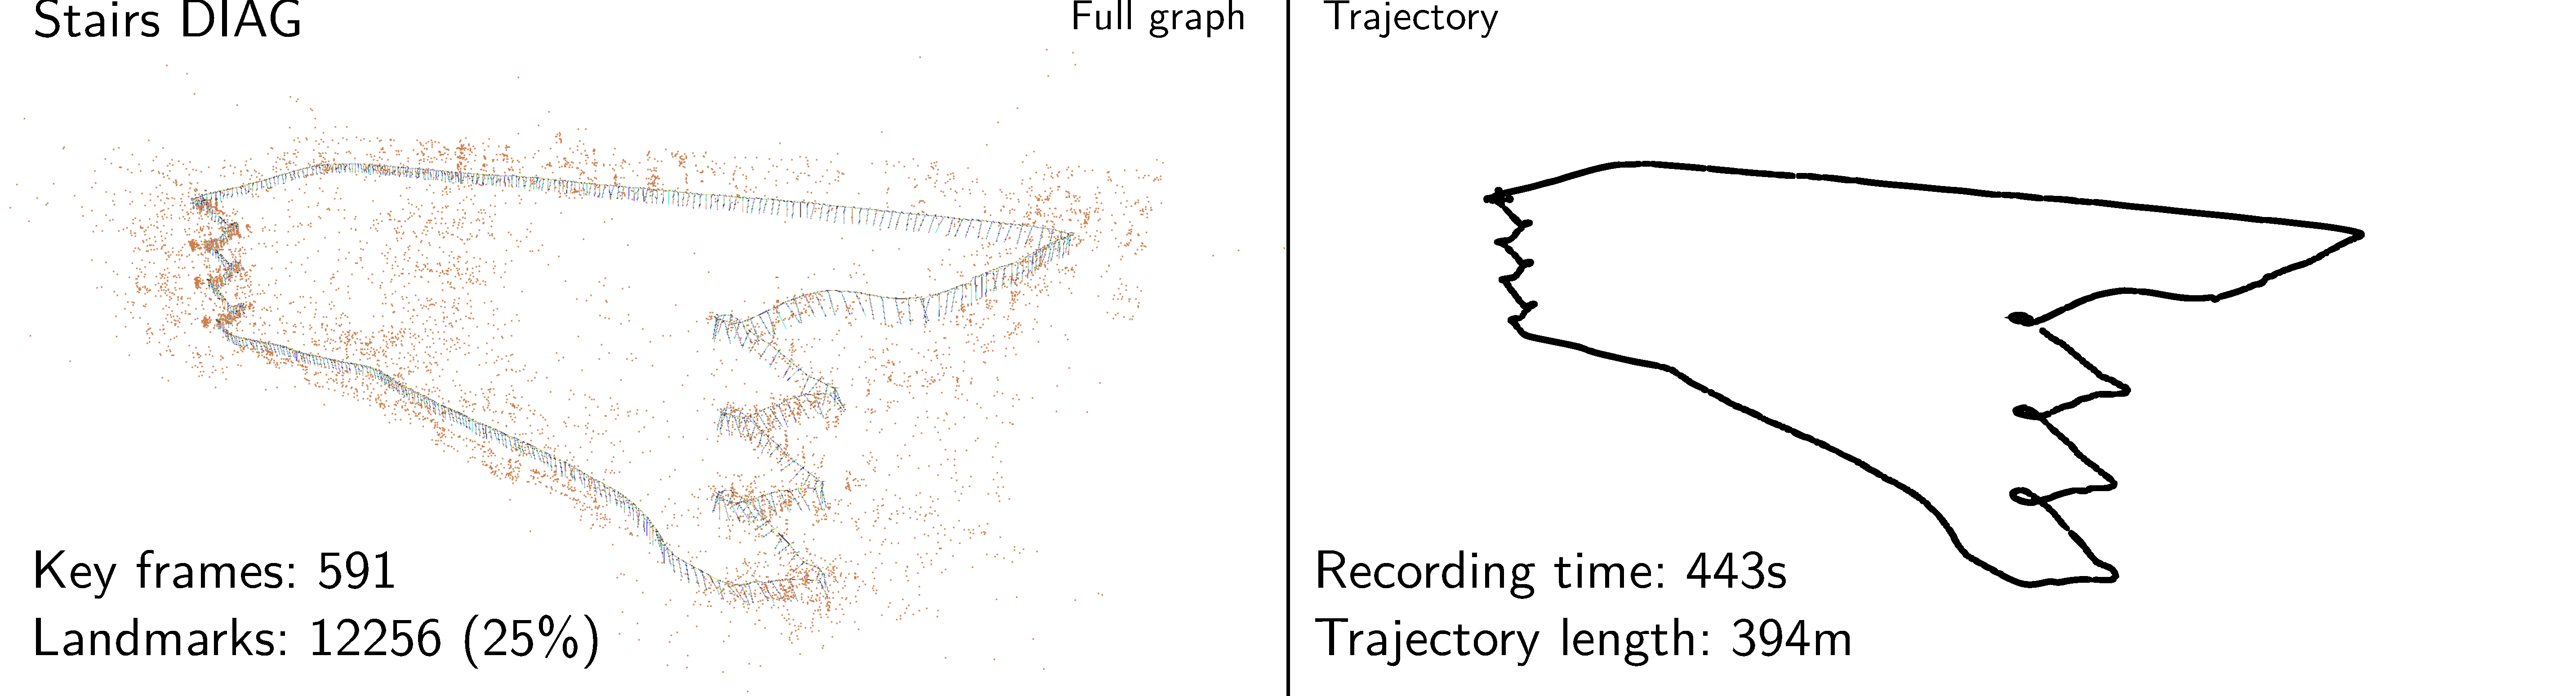
\includegraphics[width=\textwidth]{figures/results/stairs_combined.pdf}
\end{figure}
\begin{figure}[!htb]
\centering
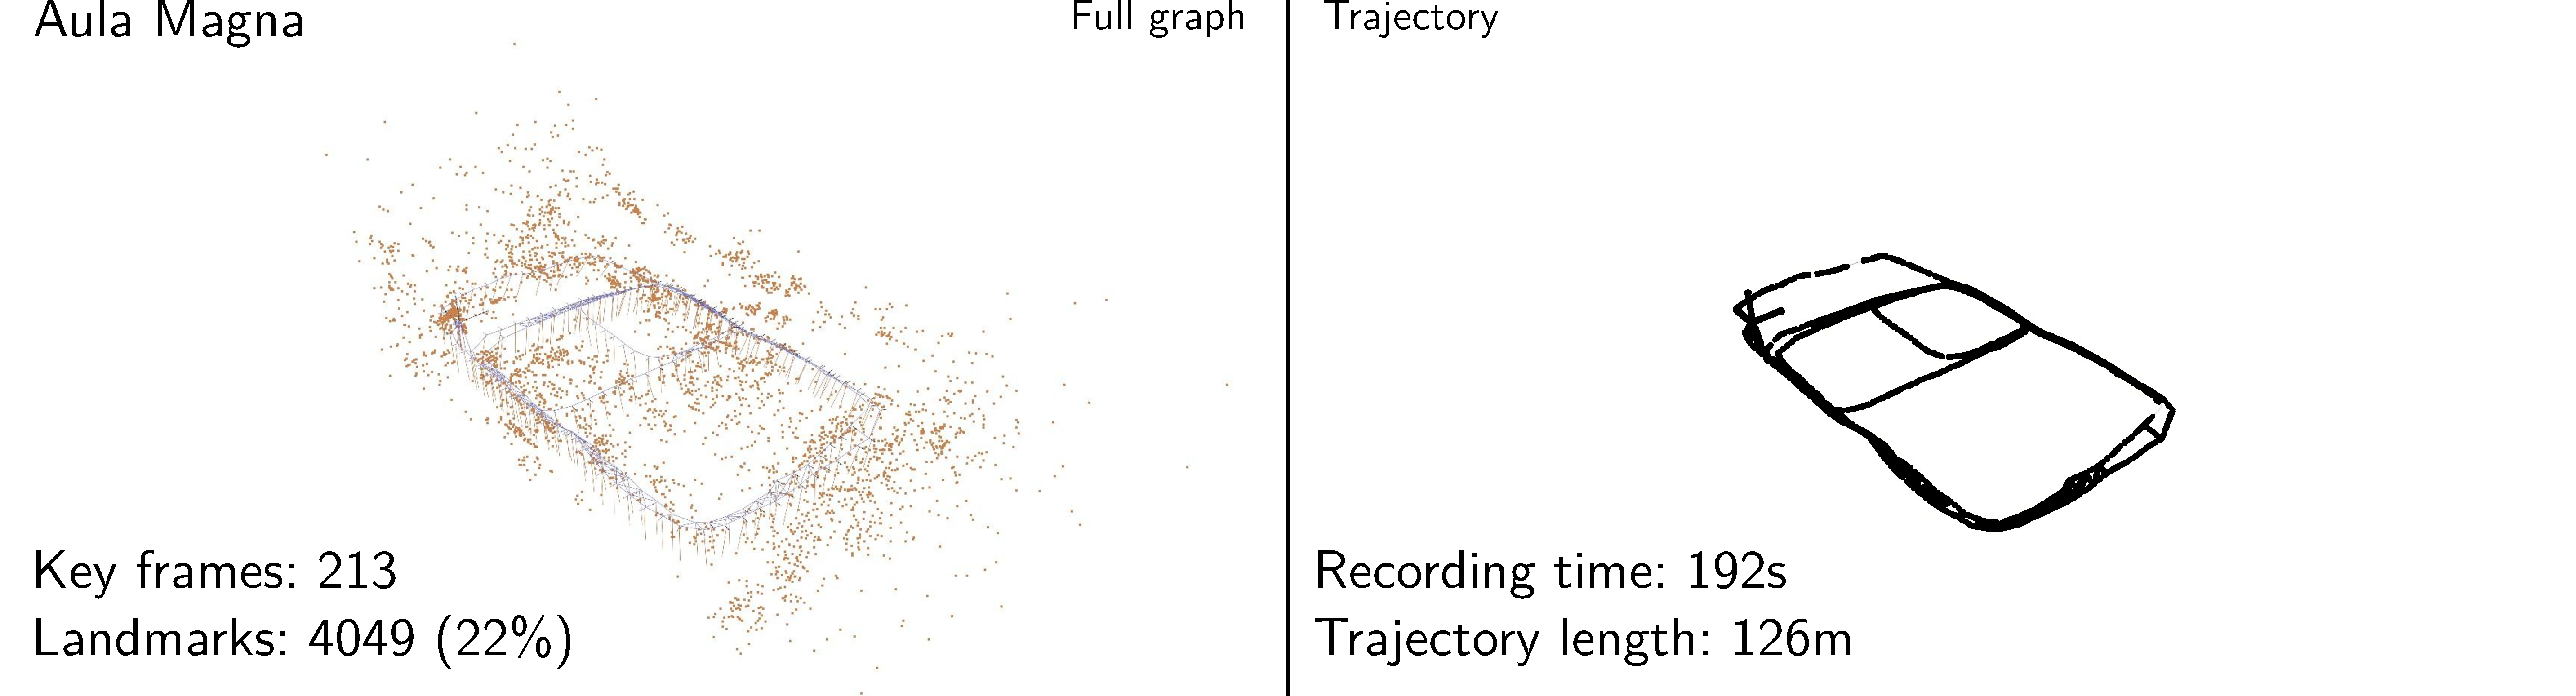
\includegraphics[width=\textwidth]{figures/results/aula_magna.pdf}
\end{figure}
\end{frame}

\begin{frame}
\frametitle{Results: bike mounted}
\begin{figure}[!htb]
\centering
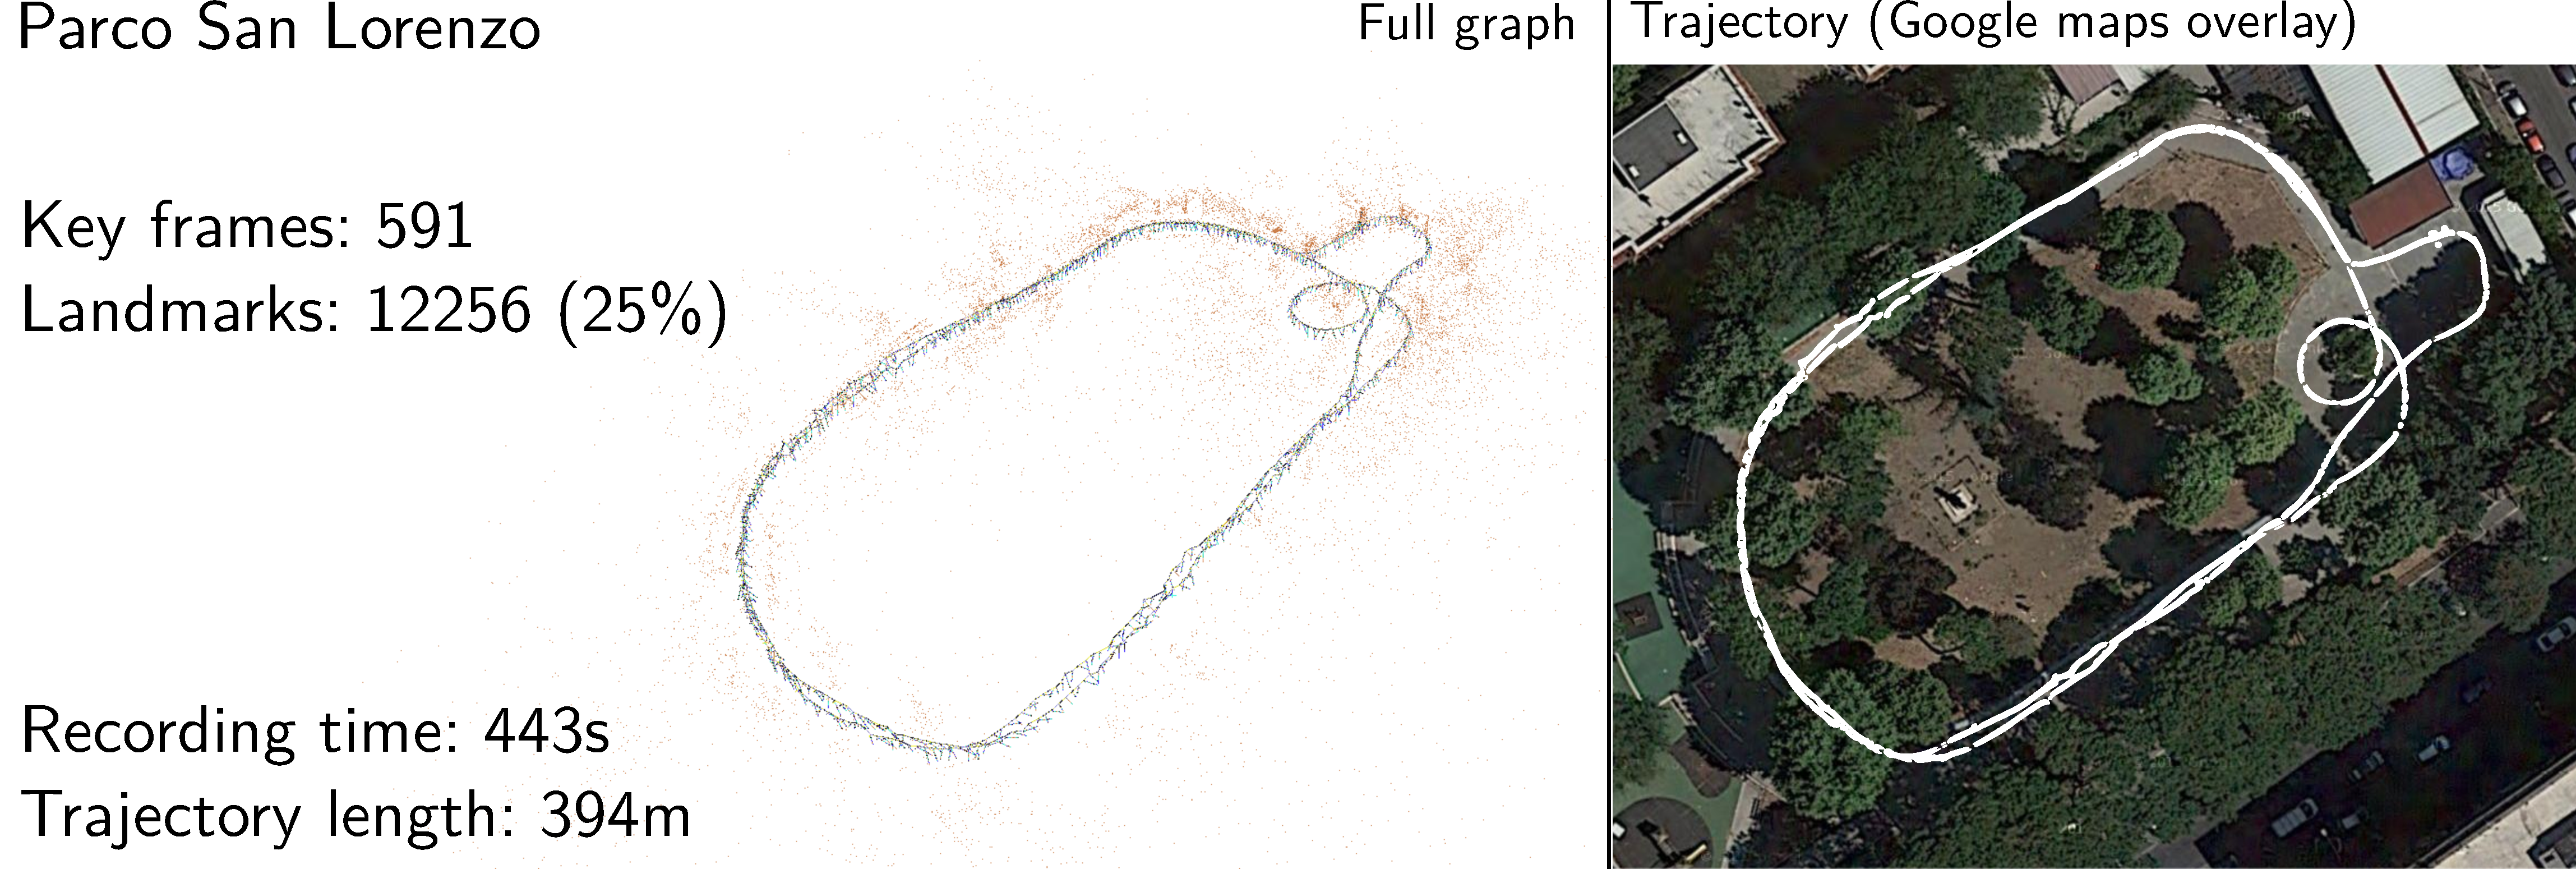
\includegraphics[width=0.8\textwidth]{figures/results/san_lorenzo_parco.pdf}
\end{figure}
\begin{figure}[!htb]
\centering
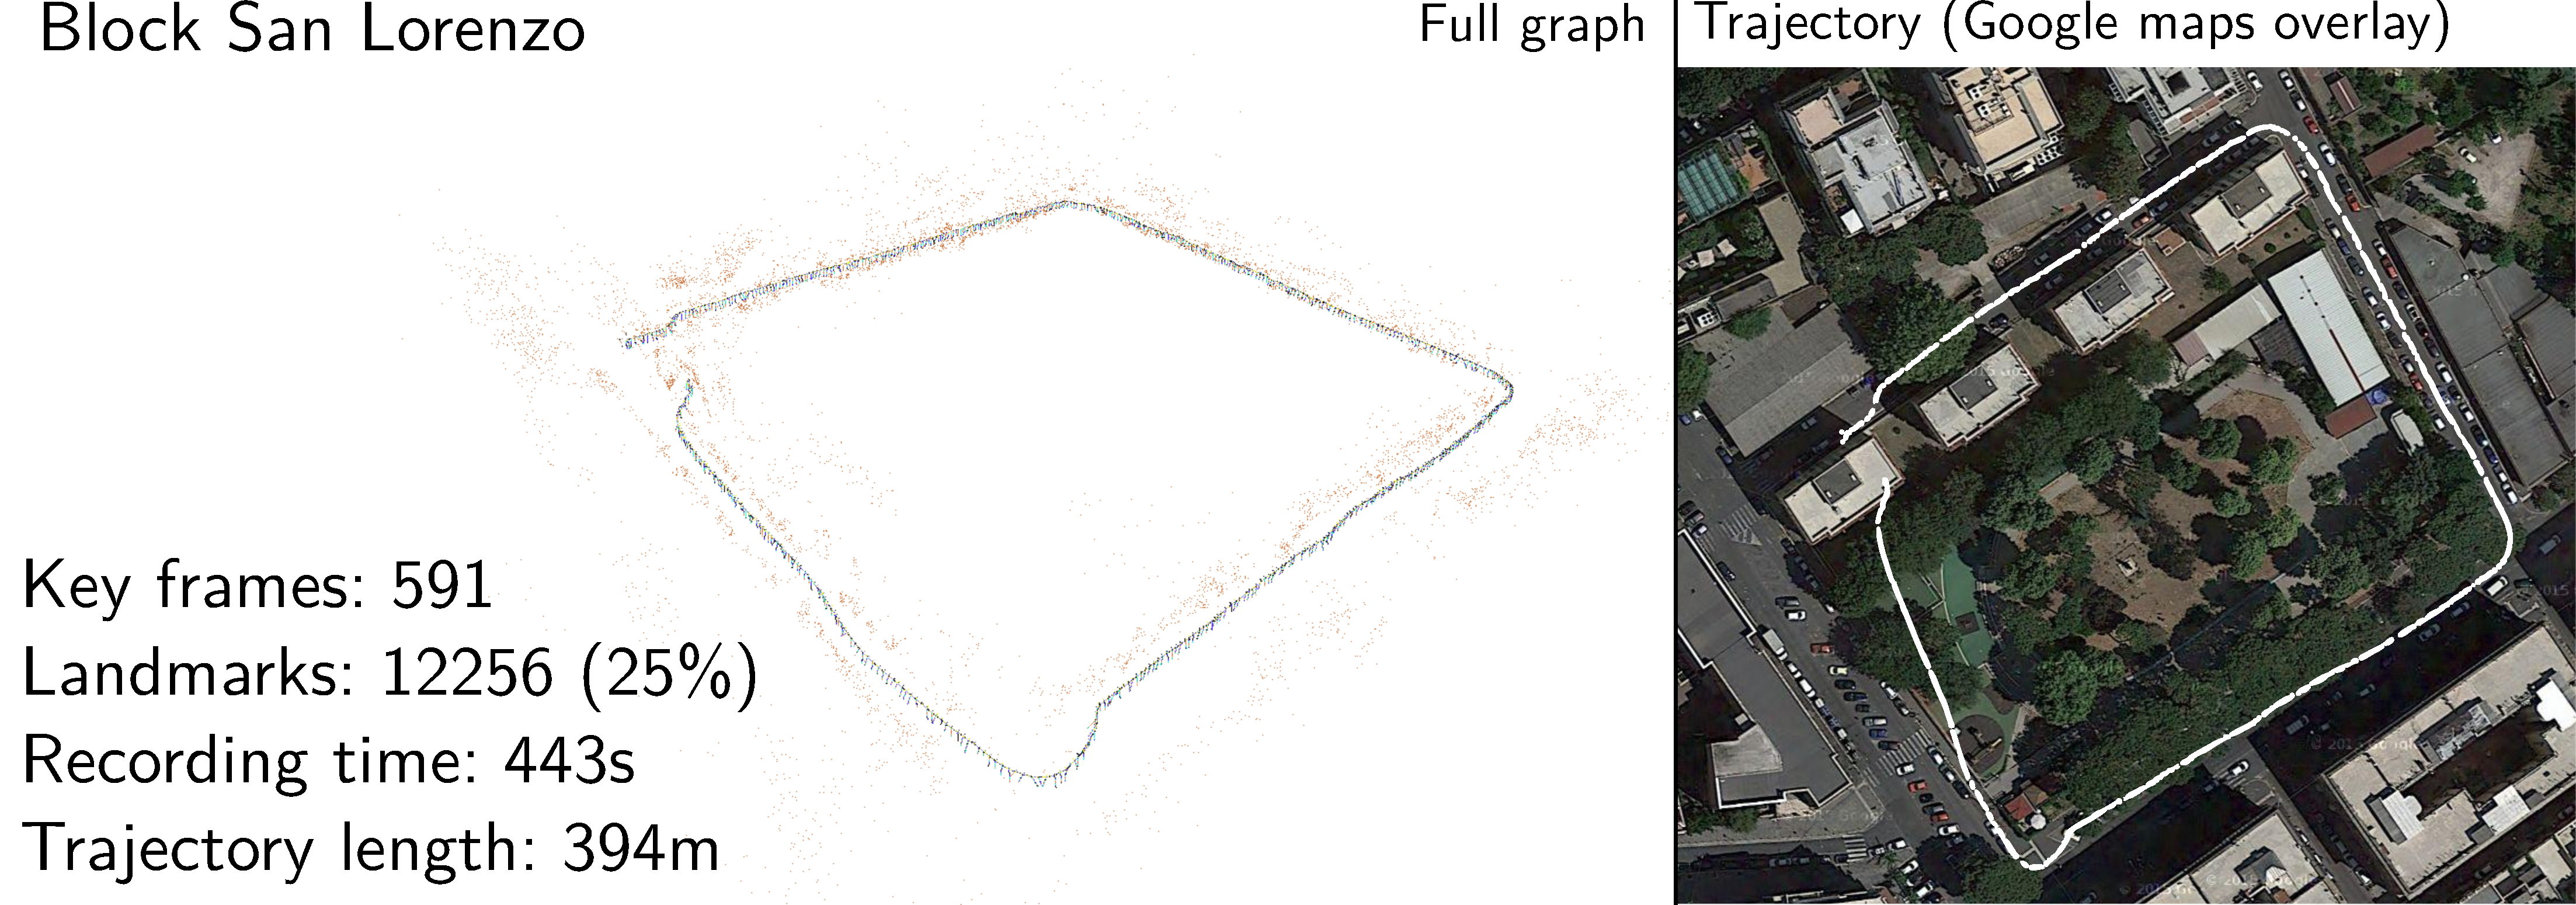
\includegraphics[width=0.8\textwidth]{figures/results/san_lorenzo_street.pdf}
\end{figure}
\end{frame}

\begin{frame}
\frametitle{Results: KITTI}
\begin{figure}[!htb]
\centering
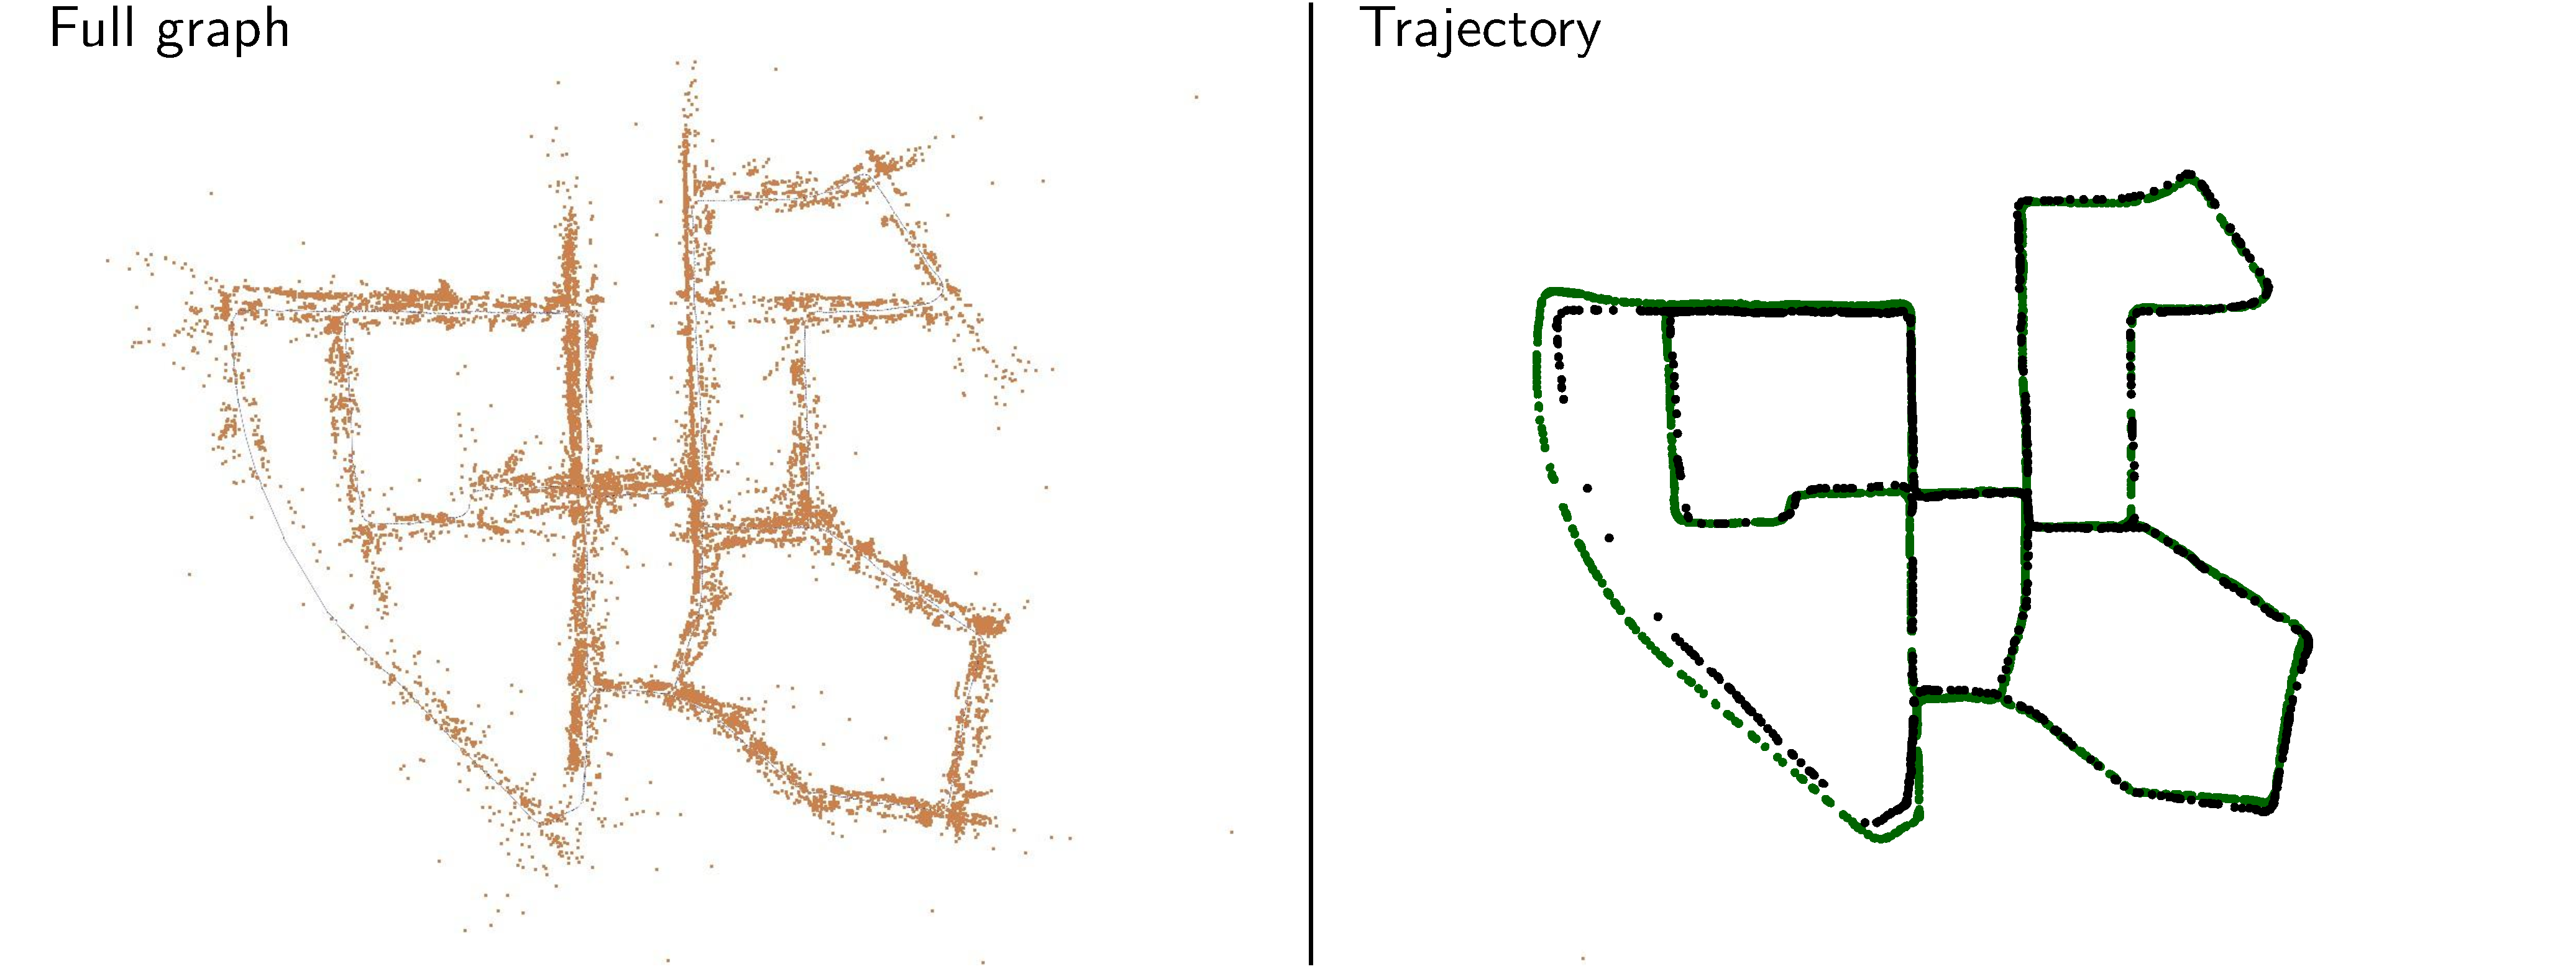
\includegraphics[width=\textwidth]{figures/results/kitti_00.pdf}
\end{figure}
\begin{figure}[!htb]
\centering
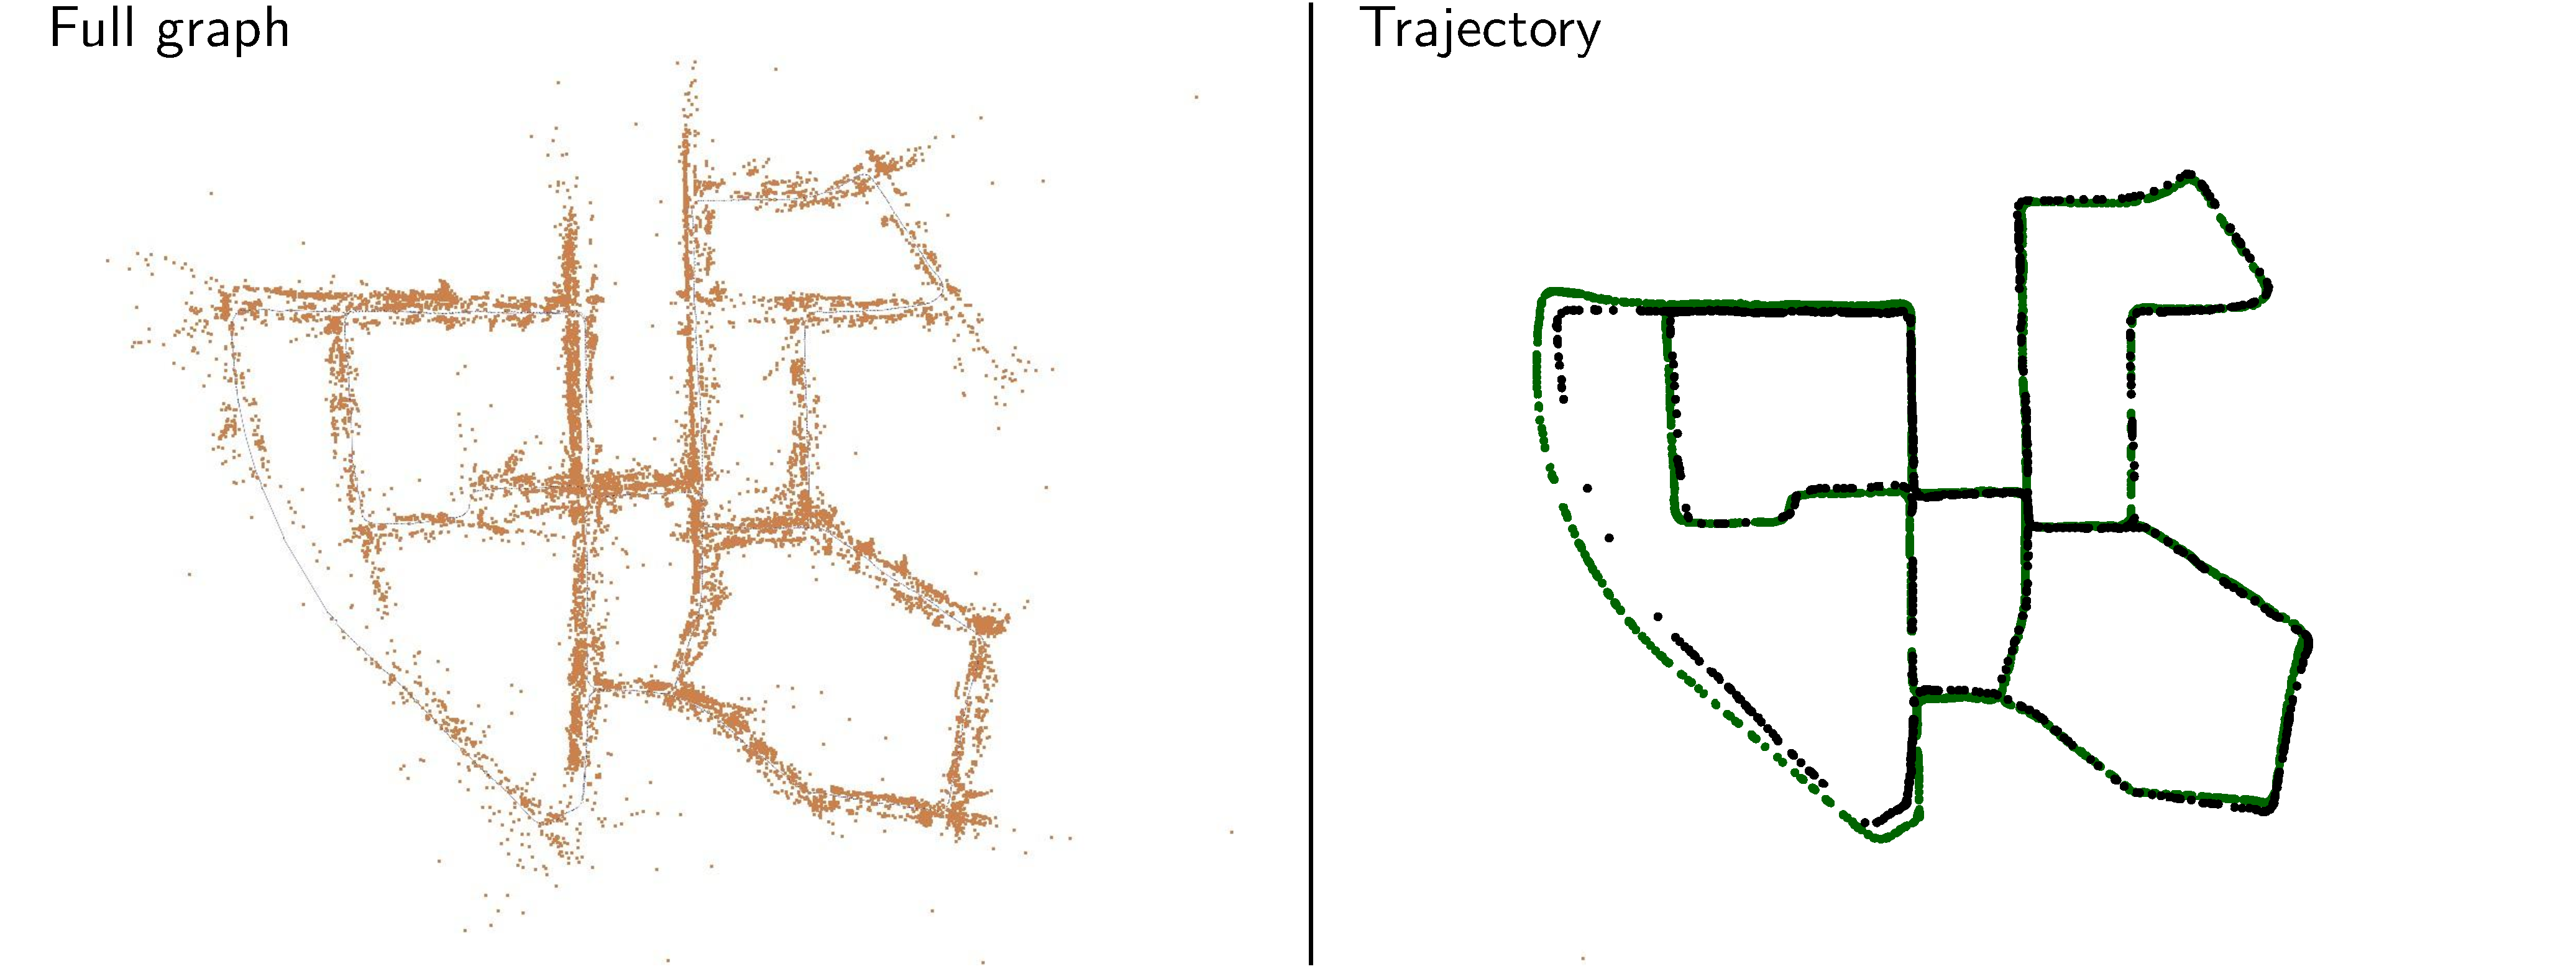
\includegraphics[width=\textwidth]{figures/results/kitti_00.pdf}
\end{figure}
\end{frame}

\begin{frame}{Conclusions and final remarks}
Regarding our final system:
\begin{itemize}
\item It works!
\item It works well
\item It works on a bike in streets and parks
\item It works without IMU
\end{itemize}
\vspace{20pt}
What could've made things faster:
\begin{itemize}
\item Start off with mocked system
\item Clear environment definition
\item Deeper read-in phase
\end{itemize}
\end{frame}

\begin{frame}{Future work}
Urgent:
\begin{itemize}
\item Filter integration (IMU)
\item Parallelization
\item Programmatic and cosmetic refactoring
\item Open source publication
\end{itemize}
\vspace{20pt}
Optional:
\begin{itemize}
\item Improved feature handling
\item Improved graph optimization
\end{itemize}
\end{frame}

\end{document}
